\relatorio
{Qualidade Educacional e Valorização Imobiliária: Um Estudo sobre o Efeito das Escolas em São Paulo}
{
    \noindent Pesquisadores: Gabriel de Araújo Alves, Phillipe Libreti Dias e Tiago Milani
    
    % \noindent Orientador: Adriano Borges Costa
}
{
    Este relatório investiga o impacto da localização de escolas sobre os preços de imóveis na cidade de São Paulo. A pesquisa examina a relação entre a proximidade de escolas e o valor médio dos imóveis, buscando identificar se a presença de escolas de alta qualidade influencia de forma significativa o mercado imobiliário na cidade. O estudo utiliza dados de preços de imóveis e informações sobre a localidade de escolas para analisar esta relação, com o objetivo de fornecer insights valiosos para compradores, vendedores e formuladores de políticas.
}
{Microeconometria, Modelagem preditiva, Previsão, Impacto, Localização, Valorização imobiliária.}

\section{Introdução}
% Na dinâmica metrópole de São Paulo, onde cada busca por um lar ideal incorpora uma teia de considerações, a proximidade de escolas emerge como um elemento central. Em uma realidade onde o tempo muitas vezes é escasso para os trabalhadores que enfrentam longos deslocamentos diários, a escolha do local de residência torna-se um delicado equilíbrio entre praticidade e qualidade de vida.

% A relevância desse cenário transcende a esfera individual, alcançando dimensões sociais e políticas. Para compradores e vendedores de imóveis, compreender como a presença de escolas próximas impacta nos preços torna-se crucial. Esse entendimento não apenas guia decisões financeiras, mas também delineia oportunidades de investimento e estratégias de mercado.

% No âmbito das políticas públicas, esse estudo lança luz sobre a intrincada relação entre a qualidade da educação, a configuração urbana e as disparidades sociais. A análise do mercado imobiliário, entrelaçada com a presença de escolas, oferece insights valiosos para orientar investimentos em infraestrutura educacional e enfrentar obstáculos potenciais na construção de habitações acessíveis.

% Essa motivação, alimentada pela curiosidade em compreender uma dinâmica tão essencial para a sociedade paulistana, guia a pesquisa que se desdobra. Ao convergir as ferramentas analíticas da microeconometria e da modelagem preditiva, nosso objetivo é desvelar os complexos matizes que permeiam as interações entre o mercado imobiliário e o setor educacional.

% Assim, neste estudo, exploramos não apenas os impactos quantitativos da localização das escolas nos preços dos imóveis, mas também aprofundamos nossa compreensão das implicações sociais e políticas subjacentes a essa interseção única.

A cidade de São Paulo é uma metrópole em constante transformação, onde a busca por um lar ideal envolve inúmeras considerações. Uma dessas considerações, particularmente importante para muitos cidadãos, é a proximidade de escolas, dado que uma grande parte dos trabalhadores se deslocam grandes distâncias até o trabalho e não tem tanto tempo para seguir com a rotina escolar de seus filhos. Dessa forma, esse artigo busca analisar o efeito das escolas sobre o preço do metro quadrado, especificamente se a existência de escolas próximas à residências eleva seus preços. 

O assunto de como a educação afeta o mercado mobiliário já é amplamente estudado, com diversos artigos abordando tanto a situação nacional como de outros países. Um deles, \citefield{chan2020valuing}{title} \cite{chan2020valuing}, busca analisar, no contexto chinês, o valor dos imóveis relacionados com a qualidade das escolas primárias. Apesar das diferenças com o contexto brasileiro, o artigo traz diversos \textit{insights} sobre como a medição do valor dos imóveis dependem de diversos fatores, tanto das características internas de cada um quanto de seus arredores.

Uma das principais metodologias, aplicada inclusive no artigo citado, é a de preços hedônicos. A análise hedônica considera que o preço de um imóvel é determinado não apenas pela sua localização, tamanho e idade, mas também por uma série de características intrínsecas, como o número de quartos e banheiros, a presença de áreas de lazer, a vista, a orientação solar e muitas outras variáveis. Cada uma dessas características tem um impacto no preço final por metro quadrado do imóvel, podendo inclusive ser capaz de quantificar o quanto cada uma dessas peculiaridades afeta o valor encontrado.

Dessa forma, o conhecimento e o estudo dos caminhos que definem os preços dos imóveis, em especial relacionado à educação, uma das necessidades essenciais de todo cidadão, será capaz de guiar tanto os estudos de qualidade de ensino e deslocamento urbano, por parte da formulação e aplicação de políticas públicas, além de assistir a tomada de decisão de compradores e vendedores que desejam auferir os preços de seus imóveis com base em aspectos escolares.

\section{Revisão da Literatura}

Antes de explorar nossos próprios dados, é relevante destacar pesquisas semelhantes em outros contextos. Por exemplo, o estudo \citefield{chan2020valuing}{title} \cite{chan2020valuing} investigou a valorização do metro quadrado de áreas residenciais segundo a qualidade das escolas primárias em áreas urbanas chinesas, com a particularidade específica do país de que a escolha da família sobre a alocação de filhos à escola não é arbitrária, sendo limitada pela região onde vivem, assim tornando a escolaridade uma alocação ao invés de uma escolha.

Além desse, outro artigo que explora a precificação de imóveis com base na existência de escolas ao seu redor é \citefield{fack2010better}{title} \cite{fack2010better}, que analisa os valores de compra e venda de imóveis que estejam a algumas distâncias de referência de escolas na cidade de Paris, indicando que eles serão os mais afetados pela existência do serviço, comparados com imóveis mais distantes.

Por fim, o último artigo utilizado para embasar nosso trabalho é o \citefield{rosen1974hedonic}{title} \cite{rosen1974hedonic}, que explora, de forma totalmente teórica, a formação de uma teoria de preços hedônicos, que seria formulada a partir tanto de preços implícitos dos compradores e vendedores, quanto da característica de equilíbrio do próprio mercado em que os bens estariam inseridos.


\section{Motivação}
% Alternativa pro comeco) O interesse em explorar o problema abordado neste relatório origina-se da importância significativa desse tópico para a sociedade paulistana.
A motivação para o problema descrito neste relatório parte da curiosidade dos pesquisadores em entender um tema altamente relevante para a sociedade paulistana. A cidade de São Paulo é uma metrópole em constante transformação, onde a busca por um lar ideal envolve inúmeras considerações. Uma dessas considerações, particularmente importante para muitos cidadãos, é a proximidade de escolas. Reforçando que uma grande parte dos trabalhadores deslocam grandes distâncias até o trabalho e não tem tanto tempo para seguir com a rotina escolar de seus filhos.

Nesse sentido, é importante destacar que questões relacionadas ao mercado imobiliário já têm sido amplamente debatidas tanto no campo da microeconometria quanto em diversos problemas de modelagem preditiva. No entanto, a combinação dessas duas abordagens de estudo, no contexto da análise do impacto da localização de escolas sobre os preços de imóveis, se revela particularmente relevante e motivadora para os pesquisadores.

A convergência dessas ferramentas analíticas permite abordar um problema de grande interesse prático de maneira abrangente e fundamentada em dados. Além disso, oferece a oportunidade de aprofundar nossa compreensão das complexas interações entre o mercado imobiliário e o setor educacional.

% \section{Relevância do problema}

% A relevância deste estudo pode ser compreendida em diversos níveis:

% \textbf{Tomada de Decisão de Compra e Venda}: Para compradores e vendedores de imóveis, entender como a localização das escolas afeta os preços é fundamental na tomada de decisão. Aqueles com famílias muitas vezes estão dispostos a pagar um prêmio por imóveis próximos a escolas de alta qualidade, enquanto investidores podem identificar oportunidades de valorização com base na localização das escolas.

% \textbf{Políticas Públicas}: Para formuladores de políticas, este estudo pode ser uma fonte valiosa de informações sobre a relação entre a qualidade da educação, a segregação urbana e as desigualdades sociais. Além disso, pode orientar o desenvolvimento de políticas de investimento em infraestrutura educacional, bem como identificar potenciais obstáculos para a construção de habitações populares.

\section{Modelo Microeconômico}

O modelo definido, baseado nas literaturas previamente vistas de \textcite{chan2020valuing}, \textcite{fack2010better} e \textcite{rosen1974hedonic} , define a utilidade do indivíduo como sendo
\begin{equation}
    U=U\{z_1,z_2,...,z_n,x\}
\end{equation}
Com \(z_n\) definindo a percepção de valor do imóvel, que possui um conjunto de características y, e x representando uma variável agregada de todos os outros bens de consumo desejados. Além disso, há uma restrição orçamentária para cada um dos indivíduos, definida pela equação
\begin{equation}
    I=x+p(z)
\end{equation}
Sendo p(z) a variável que define o preço do imóvel.

A percepção de valor do imóvel, \(z_n\), é definida por
\begin{equation}
    z_n=f(\phi_n,\epsilon_n)
\end{equation}
Com  \(\phi_n\) representando a distância até a escola mais próxima ao imóvel, e \(\epsilon_n\) sendo um vetor de outras características relevantes que ele possui, como, por exemplo, número de banheiros e a existência de ar condicionado no local. No modelo, é assumido que \(\phi_n\) é negativamente relacionado à percepção de valor dada pelo indivíduo. Quanto mais afastado o imóvel está da escola, para a maioria das pessoas, menor é a utilidade percebida pelos moradores. Consequentemente, a propriedade torna-se menos atrativa e, por conseguinte, é atribuído um valor menor a ela.

Dessa forma, ao compararmos dois imóveis, um mais distante de uma escola, e outro menos, observaríamos que, considerando todas as outras variáveis constantes, para aquele mais longe, há uma percepção de valor menor, o que, portanto, impactaria em um preço comparativamente menor àquele com uma distância menor à escola, que, dessa forma, teria um $p(z)$ maior, tudo o mais constante. Assim, podemos concluir que, segundo o modelo, a distância de imóveis até a escola, sejam elas tanto públicas quanto privadas, leva a uma valorização do valor do metro quadrado dos imóveis mais próximos em São Paulo.


\section{Base de Dados}

Este projeto combina dois conjuntos de dados essenciais para sua execução: O primeiro dataset, obtido através do site de dados da Prefeitura de São \textcite{DadosPrefeitura} (clique \href{http://dados.prefeitura.sp.gov.br/nl/dataset/cadastro-de-escolas-municipais-conveniadas-e-privadas}{\textbf{aqui}} para acessar os dados de cada ano), refere-se ao cadastro de escolas municipais, conveniadas e privadas na metrópole paulista. Este conjunto de dados inclui informações como descrição regional da escola, código da escola, diretoria e subprefeitura onde está localizada, detalhes sobre a localização (CEP, endereço, latitude e longitude) e outras variáveis pertinentes.Dessa forma, variáveis relevantes para o modelo incluem o nome da escola, o tipo de escola (pública ou privada) e, como mencionado anteriormente, as coordenadas de localização (latitude e longitude) do ambiente escolar.

O segundo conjunto de dados, disponibilizado pelo \href{https://www.kaggle.com/code/argonalyst/an-lise-business-case-ds-loft}{\textbf{Kaggle}}, é proveniente de um business case da empresa de imóveis Loft e oferece uma perspectiva detalhada sobre características específicas de propriedades, como metragem quadrada e número de quartos, além do tipo de contrato (aluguel ou venda) e do preço médio de lançamento do imóvel correspondente para cada tipo mencionado anteriormente.

Combinados, esses conjuntos de dados possibilitarão uma análise integrada do mercado imobiliário e escolar, explorando a relação entre fatores urbanos e características específicas de imóveis.

% \subsection{Tabela Dados Abertos prefeitura}
%     \subsection*{Tabela}

% \begin{table}[H]
    \centering

    
    \begin{tabular}{|m{0.25\linewidth}|m{0.20\linewidth}|}
      \hline
      \textbf{Variável} & \textbf{Descrição}  \\
      \hline
      nomesc & Nome da Escola  \\
      \hline
      Tipo & Tipo da Escola \\
      \hline
      Coordenadas & Latitude e Longitude combinados  \\
      \hline
    \end{tabular}
    \caption{Descrição das Variáveis da Base de Dados dos dados abertos prefeitura de São Paulo}
    \label{tab_variaveis-itbi}
\end{table}



% Para a tabela de escolas que se refere aos dados abertos da prefeitura de São paulo, de 2019, a base foi filtrada obtendo-se as colunas vistas acima. Nesse sentido, as variáveis mais relevantes dizem respeito a localização e o tipo de escola (privada ou publica).

\subsection{Resumo Estatístico Loft dataset}
\subsection*{Tabela}

\begin{table}[H]
    \centering

    
    \begin{tabular}{|m{0.20\linewidth}|m{0.20\linewidth}| m{0.10\linewidth}|m{0.10\linewidth}| m{0.10\linewidth}|m{0.10\linewidth}|}
      \hline
      \textbf{Variável} & \textbf{Descrição} & \textbf{Média} & \textbf{Desvio padrão}  & \textbf{Mínimo} & \textbf{Máximo} \\
      \hline
      Rooms & Número de quartos na propriedade & 2.32 & 0.715 & 1 & 6 \\
      \hline
      Toilets & Quantidade de banheiros na propriedade & 2.038 & 0.918 & 1 & 7 \\
      \hline
       Suites & Número de suítes na propriedade  & 0.9315 & 0.773 & 0 & 6 \\
      \hline
       Parking & Quantidade de vagas de estacionamento & 1.326 & 0.752 & 0 & 7 \\
      \hline
      Elevator & Quantidade de elevadores & 0.415 & 0.493 & 0 & 1 \\
      \hline
      Furnished & Se é mobiliado ou não & 0.117 & 0.322 & 0 & 1 \\
      \hline
      Swimming Pool & Se há piscina ou não no imóvel & 0.54 & 0.498 & 0 & 1 \\
      \hline
      New & Indicação de propriedade nova & 0.03 & 0.177 & 0 & 1 \\
      \hline
      District & Nome do bairro & - & - & - & - \\
      \hline
      Price per sqm & Preço por metro quadrado & 6891.64 & 3182.7 & 755.55	 & 46212.17 \\
      \hline
      Coordenadas & Latitude e Longitude & - & - & - & -\\
      \hline
    \end{tabular}
    \caption{Descrição das Variáveis da Base de Dados Da Loft filtrada}
    \label{tab_variaveis-itbi}
\end{table}



A tabela acima oferece uma visão geral das variáveis relevantes presentes na Base de Dados Loft de São Paulo. É importante destacar que os valores apresentados na tabela são aproximados e referem-se especificamente a imóveis caracterizados como tendo preço de venda. Embora a base contenha imóveis com preço de aluguel, esses foram desconsiderados para fins de análise. Essa base de dados contém informações sobre transações imobiliárias, incluindo detalhes sobre as propriedades, valores e características relevantes. As variáveis listadas nesta tabela são fundamentais para entender o conteúdo e a estrutura dos dados, além disso houve filtragem e modificação de algumas variáveis, por exemplo, a variável \textit{Price per sqm} é fruto da divisão entre as variáveis \textit{Price} e \textit{Size}, ou seja, houve a retirada de algumas variáveis e modificação de outras para constituir as variáveis desta tabela. 

% \begin{itemize}
 
%     \item Rooms: Número de quartos na propriedade. Essa variável indica a quantidade de cômodos destinados a dormitórios.

%     \item Toilets: Quantidade de banheiros na propriedade. Refere-se à quantidade total de banheiros nas edificações.

%     \item Suites: Número de suítes na propriedade. Indica a quantidade de quartos que possuem banheiro privativo.

%     \item Parking: Quantidade de vagas de garagem.

%     \item Elevator: Quantidade de elevadores.
    
%     \item Furnished: Indica se o imóvel é mobiliado ou não.
    
%     \item Swimming Pool: Indica se a propriedade possui piscina.

%     \item New: Indicação de propriedade nova.
    
%     \item District: Nome do bairro onde a propriedade está localizada.
    
%     \item Price Per Sqm: Preço médio por metro quadrado da propriedade.
%     \item Coordenadas: Coordenadas geográficas da localização do imóvel.
    
% \end{itemize}

Nesse sentido, excetuando-se as variáveis District e Coordenadas, todas as outras colunas possuem medidas-resumo que foram apresentadas na tabela anterior afim de depreender e fornecer \textit{insights} iniciais de forma estatística.


% \section{Descritiva}
Além disso, pode-se ver uma análise descritiva rápida com a imagem a seguir:

\begin{figure}[h!]
  \centering
  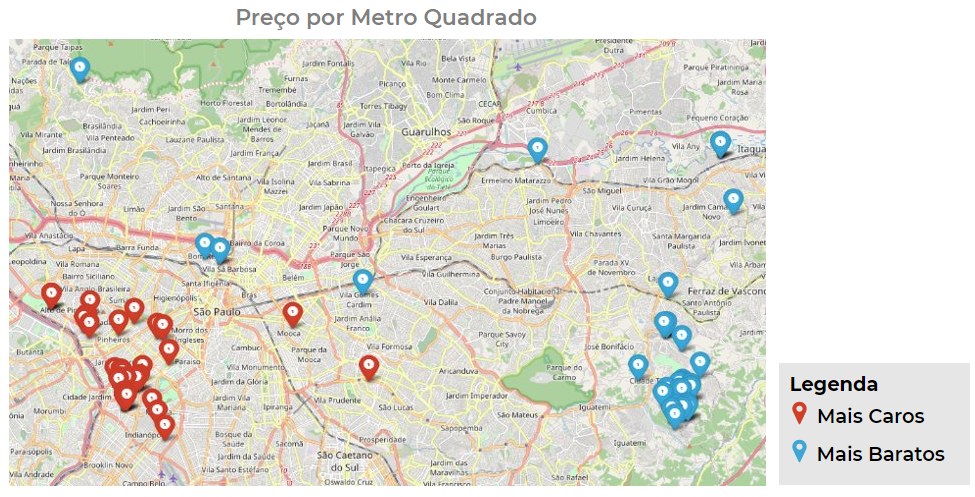
\includegraphics[width=0.8\textwidth]{relatorios/grupo6/figuras/descritiva.png} 
  \caption{Preço por metro quadrado amostra cidade São Paulo}
  \label{fig:exemplo}
\end{figure}

Na imagem anterior, a quantidade de imóveis foi reduzida, representando uma amostra de 100 unidades, composta por 50 dos imóveis mais caros e 50 dos mais baratos da base total da Loft. Isso se deve à inviabilidade computacional de gerar imagens para os mais de 6000 imóveis disponíveis na base completa.

\section{Modelo}
Este estudo visa analisar o impacto da proximidade de escolas públicas e privadas nos preços dos imóveis na cidade de São Paulo. Utilizando um modelo de regressão linear, avaliaremos como a distância até a escola mais próxima e o tipo de escola (pública ou privada) afetam o valor de mercado dos imóveis.
    
\subsection{Modelo Empirico}

A modelagem empírica leva em consideração características intrínsecas ao imóvel (número de quartos ,suítes, banheiros e características da área comum), o bairro onde o imóvel está localizado, a distância à escola mais próxima e a área do imóvel e, com isso, uma regressão linear é proposta como forma de encontrar o valor do metro quadrado para determinado imóvel, deste modo também isolando as características e similaridades entre imóveis que pudessem justificar a variação do seu preço, e isolar o efeito das escolas e si.

\paragraph{Regressao Linear}:

\vspace{0.2em}

\begin{equation}
    \frac{Preco}{m_{i}^2} = \beta_{0} + \beta_{1} \cdot distanciaescola_{i} + \beta_{2} \cdot D_{pub} + \beta_{3} \cdot Area_{i} + \beta_{4} \cdot Area_{i}^2 + \sum_{j=0}^{k} \gamma_{j} \cdot D_{bairro,j} + \sum_{p=0}^{N} \delta_{p} \cdot W_{p} + \epsilon_{i}
\end{equation}


\subsection{Descrição}
    A seguir uma secção com a explicação das variáveis:
    \begin{itemize}
        \item $distanciaescola_{i}$ :Distância do Imóvel à Escola mais próxima
        \item $D_{pub}$             :Dummy se a escola é pública ou não (valor 1 se pertence e 0 se não pertence)
        \item $Area_{i}$            :Área do Imóvel
        \item $D_{bairro,j}$        :Dummy de Bairros para identificar se determinado pertence ao bairro (valor 1 se pertence e 0 se não pertence)
        \item $W_{p}$               :Vetor de Características
            \begin{itemize}
                \item Número de Quartos
                \item Banheiros 
                \item Elevador
                \item Mobiliado ou Não
                \item Piscina
                \item Novo ou Não
         
            \end{itemize}
            
    \end{itemize}
% $\ln{Preço}_{i}=\beta_{0}+\beta_{1}*distanciaescola+\beta_{2}*escolapublica+\beta_{3}*X_{i}+\beta_{4}*X_{i}+\beta_{5}*X_{i}+\eta_{i}$


\subsection{Metodologia}

A distância até as escolas será calculada utilizando a fórmula de euler, que considera a distância entre dois pontos para estimar distâncias entre pontos definidos por coordenadas de latitude e longitude. O modelo será estimado usando o método de Mínimos Quadrados Ordinários (MQO), e a significância estatística dos coeficientes será testada para determinar quais variáveis têm um efeito significativo no preço dos imóveis. Ademais, vale ressaltar que o vetor de características e a Dummy de Bairros serão consideradas variáveis de controle afim de evitar possíveis viéses relacionados ao modelo proposto de regressão linear.

% \section{Hipotese de pesquisa}
% Espera-se que imóveis localizados mais próximos a escolas tenham um preço mais elevado, refletindo a valorização de uma maior acessibilidade a serviços educacionais. Além disso, a natureza da escola (pública ou privada) pode ter um efeito diferencial sobre o preço, possivelmente refletindo percepções sobre a qualidade da educação ou o status socioeconômico da área.


\section{Resultados}
Chegando aos resultados obtidos pela regressão estimada, observa-se, como mostrado abaixo nos principais coeficientes de análise, que se confirma os sinais demonstrados pelo modelo teórico (efeito marginal positivo para escola privada e negativo para distância à escola mais próxima).
\\

\begin{table}[h]
    \centering
    \begin{tabular}{lccc}
        \hline
        & \textbf{Coeficientes} & \textbf{P-Valor} & \\
        \hline
        \textbf{Constante} & +5308.98 [167.43] & 0.00 & *** \\
        \textbf{Distância escola mais próxima} & -0.16 [0.568] & 0.777 &  \\
        \textbf{Dummy Escola Privada} & +285.95 [111.044] & 0.010 & ** \\
        \textbf{Área} & -5.73 [1.925] & 0.003 & ** \\
        \textbf{Área\textsuperscript{2}} & +0.0238 [0.005] & 0.000 & *** \\
        \hline
    \end{tabular}
    \caption{Resultados da regressão}
    \label{tab:regressao}
\end{table}

Portanto se observa que quanto maior a distância da escola mais próxima, menor tende a ser o valor do metro quadrado do imóvel, e do mesmo modo, sendo a escola mais próxima privada, se adiciona um efeito em nível de 147.17 reais no metro quadrado. Demonstrando assim a propensão do comprador. Ademais, é notório observar que o efeito marginal de maior metragem é negativo negativo para imóveis abaixo de 118 metros quadrados, e positivo para maiores. Como segue a derivada a seguir:
\\\\
$$
\frac{\partial \frac{\text{Preço}}{m^2}}{\partial \text{Área}} = -5.73 + 0.0476 \times \text{Área}
$$
\\
Em busca de validar os resultados, realizando o teste de homocedasticidade dos resíduos se observou Homocedasticidade com 99\% de confiança.
Além disso, ao testar o mesmo modelo, porém para Preço de Aluguel por metro quadrado, se observou pouca significância nos parâmetros de interesse como demonstrado a seguir.

\begin{table}[h]
    \centering
    \begin{tabular}{lccc}
        \hline
        & \textbf{Coeficientes} &  \\
        \hline
        \textbf{Constante} & +37.05  & *** \\
        \textbf{Distância escola mais próxima} & 0.0056  & **\\
        \textbf{Dummy Escola Privada} & -1.3019  & *  \\
        \textbf{Área} & -0.1138  & *** \\
        \textbf{Área\textsuperscript{2}} & +0.0002  & *** \\
        \hline
    \end{tabular}
    \caption{Resultados da regressão para Aluguel por metro quadrado}
    \label{tab:regressao}
\end{table}



\section{Limitações}

A omissão de uma variável relevante é um ponto crítico a ser considerado na análise de transações imobiliárias. A presença ou ausência de Shoppings, Centros Culturais, Restaurantes e Comércio nas proximidades pode exercer uma influência significativa na utilidade percebida pelos agentes envolvidos. A falta de inclusão dessas variáveis pode, assim, restringir a compreensão abrangente dos fatores que impactam o cenário imobiliário.

Além disso, a heterogeneidade das preferências entre diferentes tipos de compradores e em relação a diversas características de bairros, ruas ou regiões é um aspecto crucial a ser contemplado. Considerar essas preferências distintas é fundamental para uma análise mais precisa, alinhada com a diversidade de agentes presentes no mercado imobiliário.

A detecção e tratamento de outliers são igualmente cruciais. A presença de imóveis com preços anômalos e as possíveis interferências de legislações urbanas devem ser cuidadosamente examinadas. Outliers têm o potencial de distorcer a análise estatística e levar a conclusões equivocadas, destacando a importância de uma investigação meticulosa para uma compreensão mais precisa do mercado.

Por fim, ao realizar uma análise baseada em anúncios, é imperativo reconhecer as limitações inerentes a essa abordagem. A discrepância entre os preços anunciados e os valores efetivamente transacionados pode comprometer a fidedignidade da análise. A consideração dessas variações é essencial para evitar conclusões incorretas sobre a dinâmica do mercado imobiliário.


\section{Conclusão}

Com base nos resultados obtidos, observa-se as seguintes tendências:
\vspace{0.2em}

   \begin{itemize}
      \item A longitude às escolas, em geral, sem considerar distinção entre pública e privada, está associada a uma redução de 0,16 real nos preços dos imóveis por metro quadrado para cada quilometro de distância adicional.
     \item Contrariamente, a presença de escolas privadas está associada a um aumento significativo de 285.95 reais nos preços por metro quadrado dos imóveis em relação às escolas públicas. Este aumento sugere que a proximidade a escolas privadas é um fator gerador de valor no mercado imobiliário.

   \end{itemize}
   
% Essas conclusões ressaltam a importância de considerar o tipo de instituição educacional ao avaliar os preços de imóveis em determinadas áreas. A diferenciação entre escolas públicas e privadas revela nuances importantes nas preferências dos compradores e na valorização do mercado imobiliário. Nesse sentido, para as escolas públicas na amostra analisada, não foi observada uma significância expressiva em relação à mudança no valor do metro quadrado, ao contrário do que foi evidenciado para as escolas privadas, conforme mencionado anteriormente.Ademais, o dataset de escolas tem uma quantidade maior de escolas privadas em detrimento de públicas o que pode enviesar o modelo a sugerir valorização imobiliária maior, considerando escolas privadas em detrimento de escolas públicas.
Essas conclusões ressaltam a importância de considerar o tipo de instituição educacional ao avaliar os preços de imóveis em determinadas áreas. A diferenciação entre escolas públicas e privadas revela nuances significativas nas preferências dos compradores e na dinâmica do mercado imobiliário.

No entanto, é crucial observar que, na amostra analisada, não se observou uma significância expressiva em relação à mudança no valor do metro quadrado para as escolas públicas. Em contraste, para as escolas privadas, a associação positiva entre sua presença e a valorização imobiliária é notável, como mencionado anteriormente.

Além disso, é relevante apontar que o desbalanceamento no número de escolas, favorecendo as privadas no conjunto de dados, pode introduzir um viés no modelo, levando a uma sugestão potencialmente inflada de valorização imobiliária, especialmente ao considerar escolas privadas em detrimento das públicas. Essa ponderação é crucial para uma interpretação precisa dos resultados e destaca a importância de abordar possíveis desequilíbrios na representação das escolas na amostra.

\printbibliography[keyword = {escolas}]

% \section{Próximos passos}

% \begin{itemize}
%     \item Inclusão de Variáveis Relevantes:Recomenda-se a expansão do conjunto de dados para incluir variáveis cruciais, como a presença de Shoppings, Centros Culturais, Restaurantes e Comércio nas proximidades. Essas informações podem fornecer uma compreensão mais abrangente dos fatores que influenciam as transações imobiliárias.
%     \item Consideração das Preferências Heterogêneas:Dada a identificação de preferências não homogêneas entre diferentes tipos de compradores e características específicas de bairros, ruas ou regiões, sugere-se uma análise mais aprofundada dessas preferências. Estratificar a análise de acordo com esses segmentos pode revelar insights valiosos para estratégias de precificação e marketing.
%     \item Tratamento de Outliers e Legislações Urbanas:Um próximo passo importante é realizar uma investigação detalhada sobre a presença de outliers nos preços dos imóveis e considerar o possível impacto de legislações urbanas. Lidar adequadamente com esses elementos garantirá uma análise estatística mais confiável e conclusões mais precisas.
%     \item Validação da Análise Baseada em Anúncios:Para validar a análise centrada nos preços anunciados, sugere-se a comparação com dados reais de transações efetivas. Isso ajudará a compreender melhor como as variações entre anúncios e transações podem influenciar as conclusões e proporcionar uma visão mais alinhada com a dinâmica do mercado.
%     \item Exploração de Novas Variáveis:A exploração de variáveis adicionais, como a presença de áreas verdes, infraestrutura de transporte e índices de segurança, pode enriquecer ainda mais a análise, oferecendo insights adicionais sobre os determinantes dos preços imobiliários.
 
% \end{itemize}

% \section{Referências Bibliográficas}
% \begin{itemize}

%     \item Chan, J., Fang, X., Wang, Z., et al. (2020). Valuing primary schools in urban China. Journal of Urban Economics, Link.
    
%     \item Ou, Y., Zheng, S., e Nam, K. M. (2022). Impacts of air pollution on urban housing prices in China. Journal of Housing and the Built Environment, 37(1), 423-441.
    
%     \item Zheng, S., Cao, J., Kahn, M. E., e Sun, C. (2014). Real estate valuation and cross-boundary air pollution externalities: evidence from Chinese cities. The Journal of Real Estate Finance and Economics, 48(3), 398-414.
    
%     \item Zheng, S., e Kahn, M. E. (2008). Land and residential property markets in a booming economy: New evidence from Beijing. Journal of Urban Economics, 63(2), 743-757
    
%     \item http://www.usp.br/nereus/?p=880 , Capital Humano e Capital Urbano: o Impacto das Escolas nos Preços dos Imóveis no Município de São Paulo
    
%     \item http://dados.prefeitura.sp.gov.br/nl/dataset/cadastro-de-escolas-municipais-conveniadas-e-privadas
%     \item https://www.kaggle.com/code/argonalyst/an-lise-business-case-ds-loft
% \end{itemize}




